\section{CALM Analysis}
Bloom programs define unordered collections and statements that describe
transformations over these collections.  A Bloom program may be viewed as a
dataflow graph with external inputs and outputs as sources and sinks,
respectively, collections as internal nodes, and rules as edges.  Given this
view, we may adapt powerful static analyses from the logic programming
literature which are expressed as properties of such dataflow graphs.

In this section, we implement a simple key-value store in Bud and analyze the
resulting dataflow graph.  We begin with an interface for an abstract store, and
extend it first into a single-site implementation and finally into a replicated implementation.
Along the way, we use a dataflow visualization to reason about the completeness
and correctness of the evolving program.

% TODO: tee-up points of order
% TODO: tee-up divergence into PDGs

\subsection{Predicate Dependency Graphs}
\begin{figure}[t]
\centering
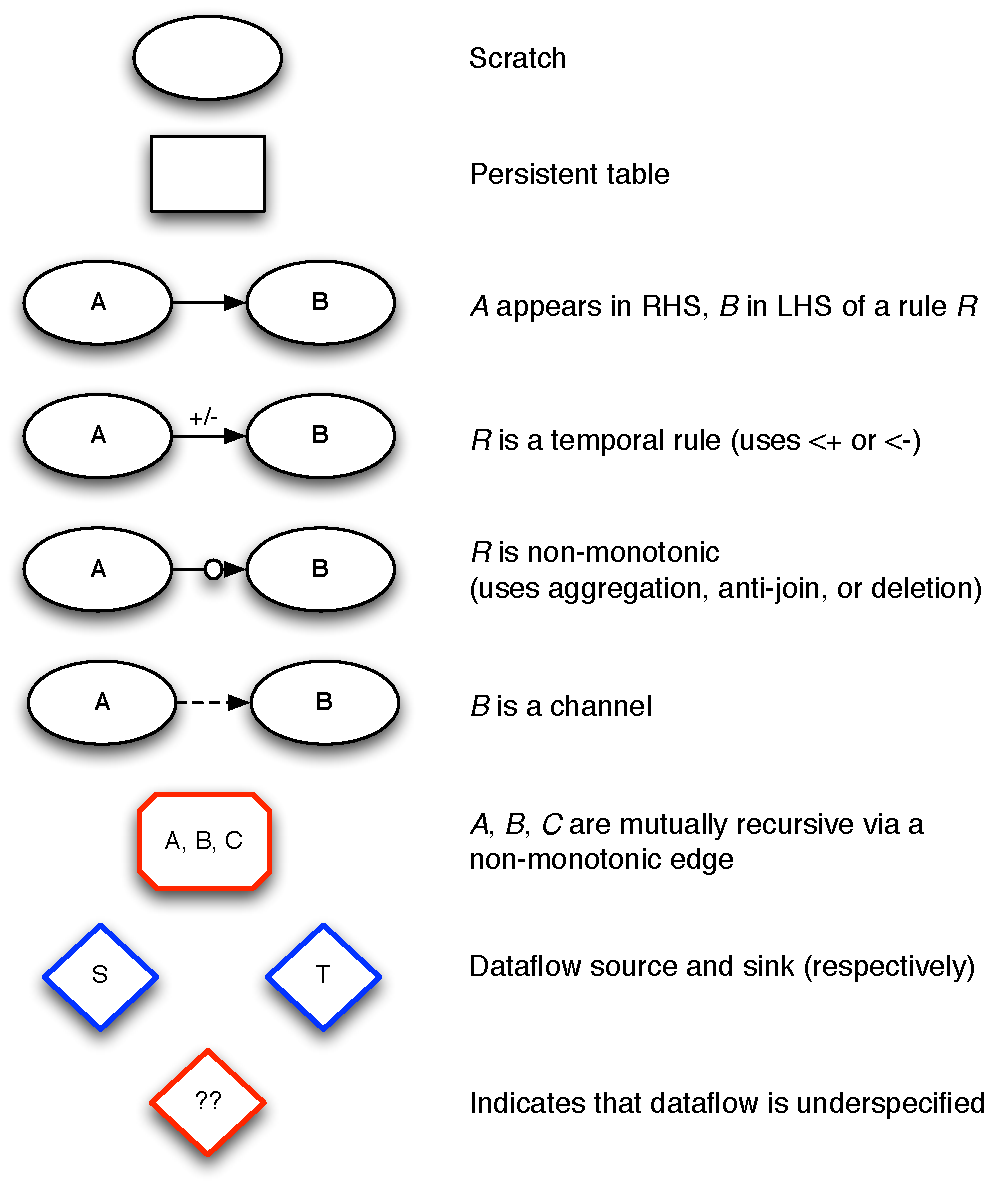
\includegraphics[width=0.9\linewidth]{fig/mittalk_legend.pdf}
\vspace{-10pt}
\caption{Visual analysis legend.}
\label{fig:analysis-legend}
\vspace{-2pt}
\end{figure}

The Bud interpreter can automatically generate a graph that represents the
dependencies between collections in a program. Each node in the graph is either
a collection or a cluster of collections; tables are shown as rectangles,
ephemeral collections (scratch, periodic and channel) are depicted as ovals, and
clusters (described below) as octagons.

A directed edge from node $A$ to node $B$ indicates that $B$ appears in the lhs
of a Bloom rule with $A$ referenced directly, or through a join expression, in
the rhs.  An edge is annotated based on the operator symbol in the rule. If the
rule uses the \texttt{$<$+} or \texttt{$<$-} operators, the edge is marked with
$+$. This indicates that facts traversing the edge ``spend'' a timestep to move
from the rhs to the lhs. Similarly, if the rule uses the \texttt{$<\sim$}
operator, the edge is a dashed line---this indicates that facts from the rhs
appear at the lhs at a non-deterministic future time. If the rule involves a
nonmonotonic operation (aggregation, anti-join, or the \texttt{$<$-} operator),
then the edge is marked with a small circle.  To make the visualizations more
readable, any strongly connected component marked with both a circle and a $+$
edge is collapsed into an octagonal ``temporal cluster,'' which can be viewed
abstractly as a single, nonmonotonic node in the dataflow. \emph{Points of
  order} are indicated in the graph by an edge with a white circle.  Any
nonmonotonic edge in the graph is a point of order, as are all edges incident to
a temporal cluster, including any self-edges.  Figure~\ref{fig:analysis-legend}
provides a legend for the analysis visualizations.

\subsection{KVS Interface}

\begin{figure}[t]
\begin{scriptsize}
\begin{lstlisting}
module KVSProtocol
  def state
    interface input, :kvput, 
      ['client', 'key', 'reqid'], ['value']
    interface input, :kvget, ['reqid'], ['key']
    interface output, :kvget_response, 
      ['reqid'], ['key', 'value']
  end
end
\end{lstlisting}
\centering
%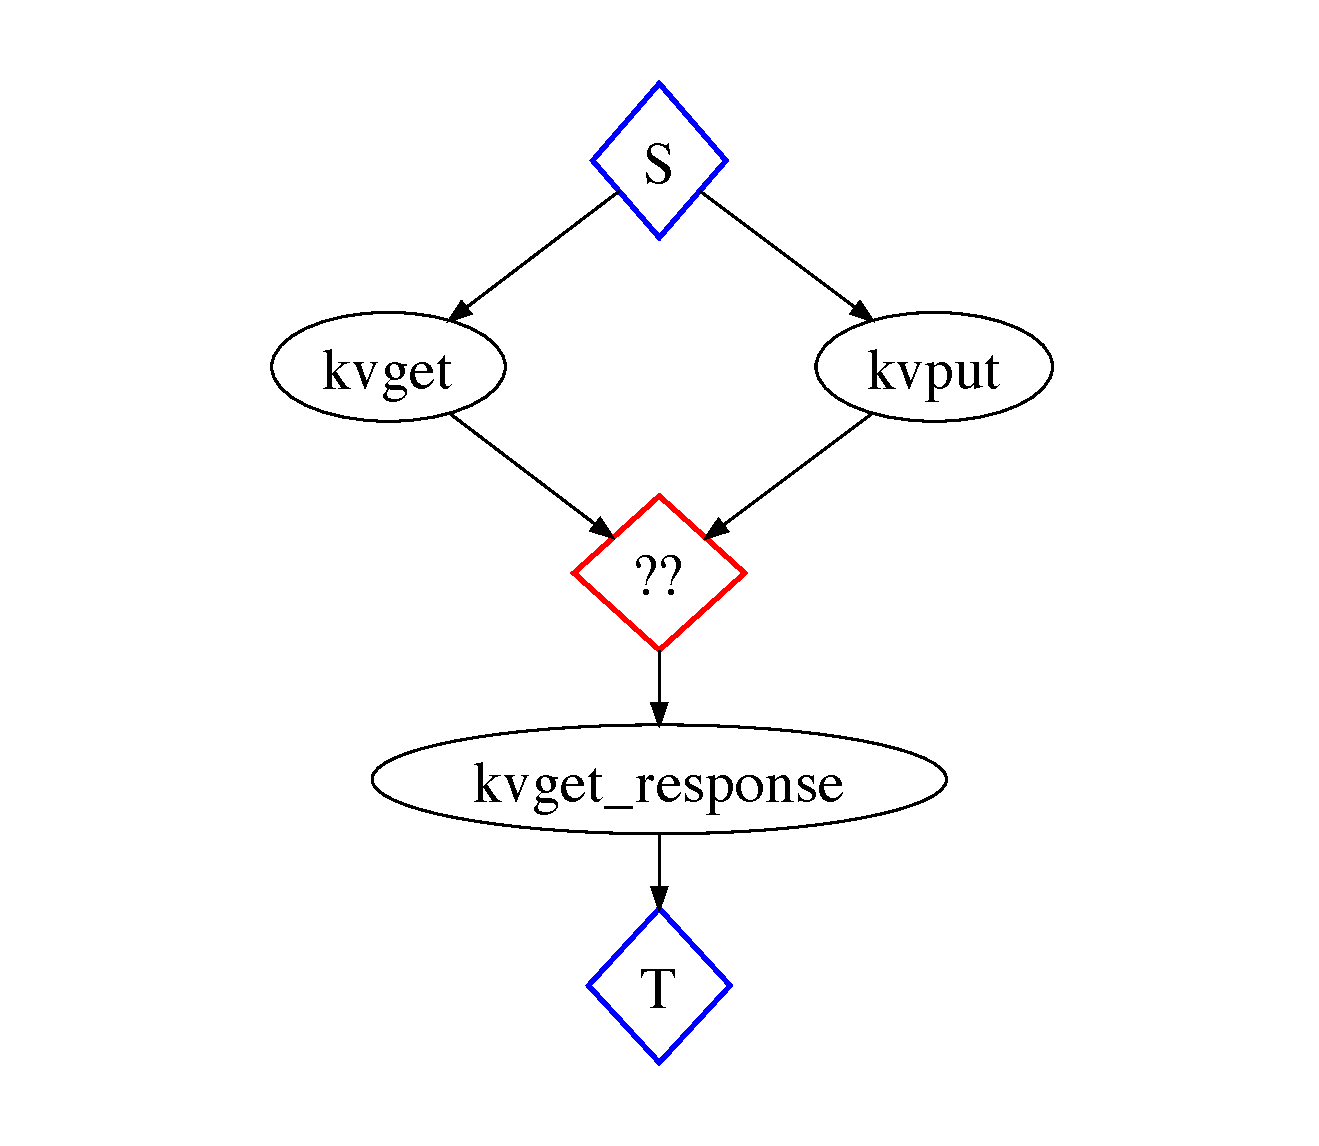
\includegraphics[width=0.4\linewidth]{fig/kvs_proto_pdg.pdf}
\vspace{-10pt}
\caption{Key-value store protocol.}
\label{fig:kvs-proto}
\end{scriptsize}
\vspace{-2pt}
\end{figure}

Figure~\ref{fig:kvs-proto} specifies a protocol for interacting with an abstract
key-value store. The protocol comprises two input events (representing attempts
to insert and fetch items from the store), and a single output event (which
represents the outcome of a fetch operation). To use an implementation of this
protocol, a Bloom program can store key-value pairs by inserting facts into
\texttt{kvput}, and can retrieve the value associated with a key by inserting a
fact into \texttt{kvget} and reading the response tuple that should eventually
appear in \texttt{kvget\_response}. In each case, the client program must supply
a unique request identifier (\texttt{reqid}) to differentiate tuples in the
event of multiple concurrent requests.  A module which uses a key-value store
but is indifferent to the specifics of the implementation may simply mix in this
protocol specification and postpone committing to a particular implementation
until runtime. As we will see shortly, an implementation of the
\texttt{KVSProtocol} is a collection of Bud rules that read tuples from the
protocol's input interfaces and send results to the output interface.

\subsection{KVS Implementation}
\begin{figure}[t]
\begin{scriptsize}
\begin{lstlisting}
module BasicKVS
  include KVSProtocol

  def state
    table :kvstate, ['key'], ['value'] (*\label{line:kvs-state}*)
  end

  declare
  def mutate
    kvstate <+ kvput.map {|p| [p.key, p.value]} (*\label{line:kvs-put}*)
    jst = join [kvstate, kvput], [kvstate.key, kvput.key] (*\label{line:kvs-join}*)
    kvstate <- jst.map {|b, p| b} (*\label{line:kvs-clean}*)
  end

  declare
  def get
    getj = join [kvget, kvstate], [kvget.key, kvstate.key] (*\label{line:kvs-getjoin}*)
    kvget_response <= getj.map do |g, t|
      [g.reqid, t.key, t.value]
    end
  end
end
\end{lstlisting}
\centering
%%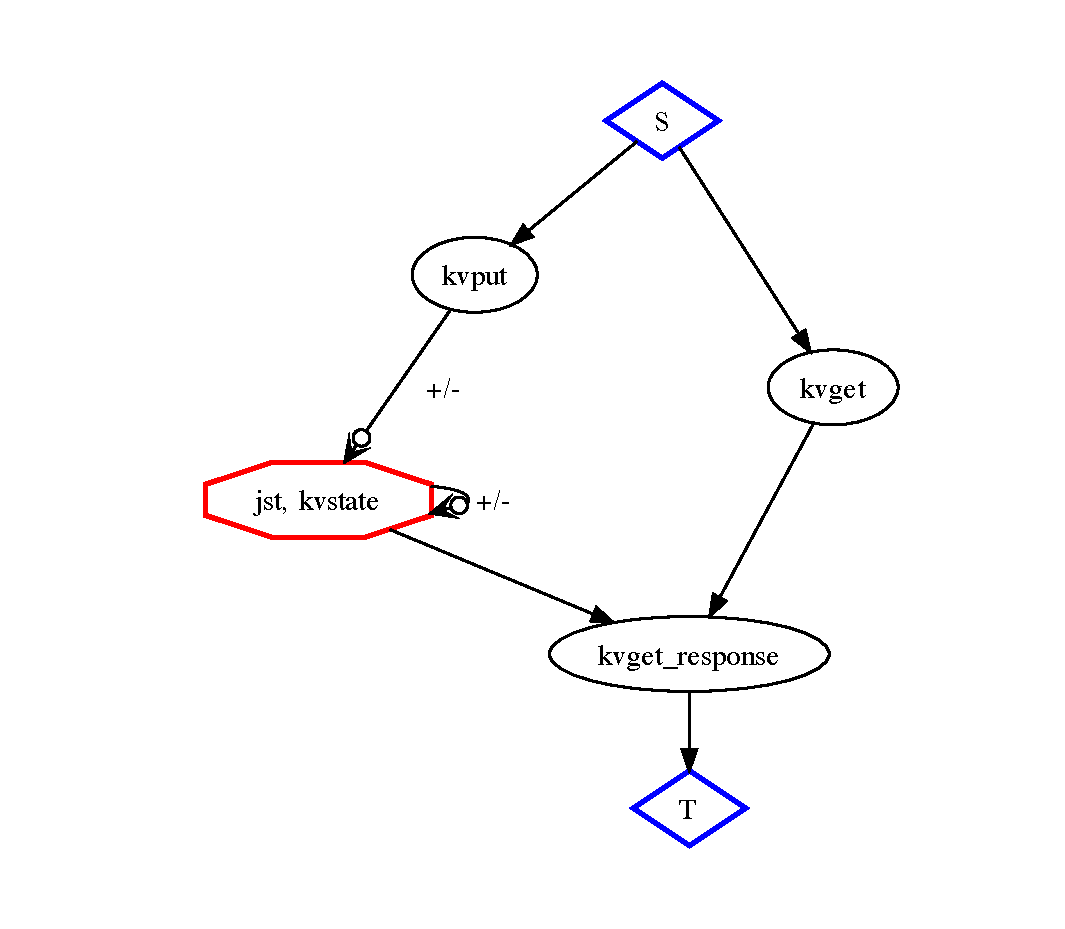
\includegraphics[width=0.55\linewidth]{fig/basickvs.pdf}
\vspace{-10pt}
\caption{Single-site key-value store implementation.}
\label{fig:kvs-impl}
\end{scriptsize}
\vspace{-2pt}
\end{figure}

Figure~\ref{fig:kvs-impl} completes the specification by supplying a very simple
realization of a key-value store.  Line~\ref{line:kvs-state} declares a table
called \texttt{kvstate} that contains the internal, persistent state of the
store.  When a \texttt{kvput} tuple appears, its key-value pair is placed in
\texttt{kvstate} in the immediate next timestep (line~\ref{line:kvs-put}).  If
a value for the given key already exists in \texttt{kvstate}, we wish to
replace it with the newer value.  Line~\ref{line:kvs-join} joins the input
interface with the internal state: if a row already exists for the current key,
the join collection \texttt{jst} will contain a tuple that is the concatenation
of the matching tuples from \texttt{kvstate} and \texttt{kvput}.  In this
event, line~\ref{line:kvs-clean} states that in the immediate next timestep (and
hence concurrently with the appearance of the new tuple derived at
line~\ref{line:kvs-put}), the old value associated with the given key does not
exist in \texttt{kvstate}.


\subsection{Replicated KVS implementation}
\begin{figure}[t]
\begin{scriptsize}
\begin{lstlisting}
module ReplicatedKVS
  include BasicKVS
  include MulticastProtocol

  def state
    interface input, :kvput, 
      ['client', 'key', 'reqid'], ['value']  (*\label{line:rep-put}*)
  end

  declare
  def local_indir
    send_mcast <= kvput.map do |k| (*\label{line:send-mcast-beg}*)
      unless members.include? [k.client]  (*\label{line:not-rep}*)
        [k.reqid, [@addy, k.key, k.reqid, k.value]]   (*\label{line:marshall}*)            
      end
    end (*\label{line:send-mcast-end}*)
    
    kvput <= mcast_done.map{|m| m.payload}  (*\label{line:mcast-done}*)

    kvput <= pipe_chan.map do |d| (*\label{line:mcast-peer-beg}*)
      if d.payload.fetch(1) != @addy
        d.payload
      end
    end (*\label{line:mcast-peer-end}*)
  end
end
\end{lstlisting}
\vspace{-10pt}
\caption{Replicated key-value store implementation.}
\label{fig:kvs-repl}
\end{scriptsize}
\vspace{-2pt}
\end{figure}


Figure~\ref{fig:kvs-repl} extends the basic KVS module to support replication of
the store state.  It does so by mixing in MulticastProtocol, which provides the
input interface \texttt{send\_mcast} and the output interface
\texttt{mcast\_done}.  Line~\ref{line:rep-put} declares an additional input
interface (\texttt{kvput}) with the same name as the input interface of the
mixed in module BasicKVS.  This allows the writer of ReplicatedKVS to interpose
additional logic between calls to KVSProtocol's input interface and the now
``protected'' input interface of BasicKVS.  In ReplicatedKVS, references to
\texttt{kvput} appearing in the LHS of rules are resolved to the \texttt{kvput}
provided by BasicKVS, while references in the RHS of rules resolve to the local
\texttt{kvput}.  Note that this is unambiguous, because it is meaningless for a
module to insert into its own input or to read data from its own output
interfaces.

Thus, lines~\ref{line:send-mcast-beg}--\ref{line:send-mcast-end} ensure that when an external caller inserts a tuple into
\texttt{kvput}, its contents are marshalled (line~\ref{line:marshall}) into \texttt{send\_mcast}
if the originating address is not another replica (line~\ref{line:not-rep}), as this would indicate
that the current replica is not the master for this update.  
The internal
\texttt{kvput} interface of BasicKVS is stimulated in one of two cases: if multicast succeeds
at the master replica (line~\ref{line:mcast-done}), or whenever a multicast is received at 
a peer replica (lines~\ref{line:mcast-peer-beg}--\ref{line:mcast-peer-end}).

\subsection{Analyses}
Figure~\ref{fig:pdg-kvs-proto-analysis} presents a visual representation of the KVS protocol.  Data
flows from the source node (an external caller) to one or both of \texttt{kvput} and 
\texttt{kvget}, through some unknown dataflow, to \texttt{kvget\_response}.
The existence of the red diamond labeled ``??'' indicates that the dataflow is underspecified:
is must be ``completed'' by supplying dataflow that, at minimum, connects the input 
interfaces to the output interface.

Figure~\ref{fig:pdg-kvs-analysis} shows the visual analysis of the basic KVS
implementation, which supplies a concrete dataflow for the unspecified component
in the previous graph.  \texttt{kvstate} and \texttt{jst} are collapsed into a
red octagon because they are part of a strongly connected component in the graph
with both negative and temporal edges.  Any data flowing from \texttt{kvput} to
the sink must cross at least one nonmonotonic point of order (at ingress to the
octagon) and possible an arbitrary number of them (via the octagon's self-edge),
and any path from \texttt{kvget} to the sink must join state potentially
affected by nonmonotonicity (because \texttt{kvstate} is used to derive
\texttt{kvget\_response}).

Reviewing the code in Figure~\ref{fig:kvs-impl}, we see that this is
unavoidable.  The contents of \texttt{kvstate} at a given time are defined (in
part; line~\ref{line:kvs-clean}) in terms of its contents at the immediate
previous state and the current input.  Hence the state of \texttt{kvstate} at
any point in time may depend on the order of arrival of \texttt{kvput} tuples.
% We challenge the reader to implement the KeyValueProto interface in a way that
% has no such point of order.



\begin{figure}[t]
\centering
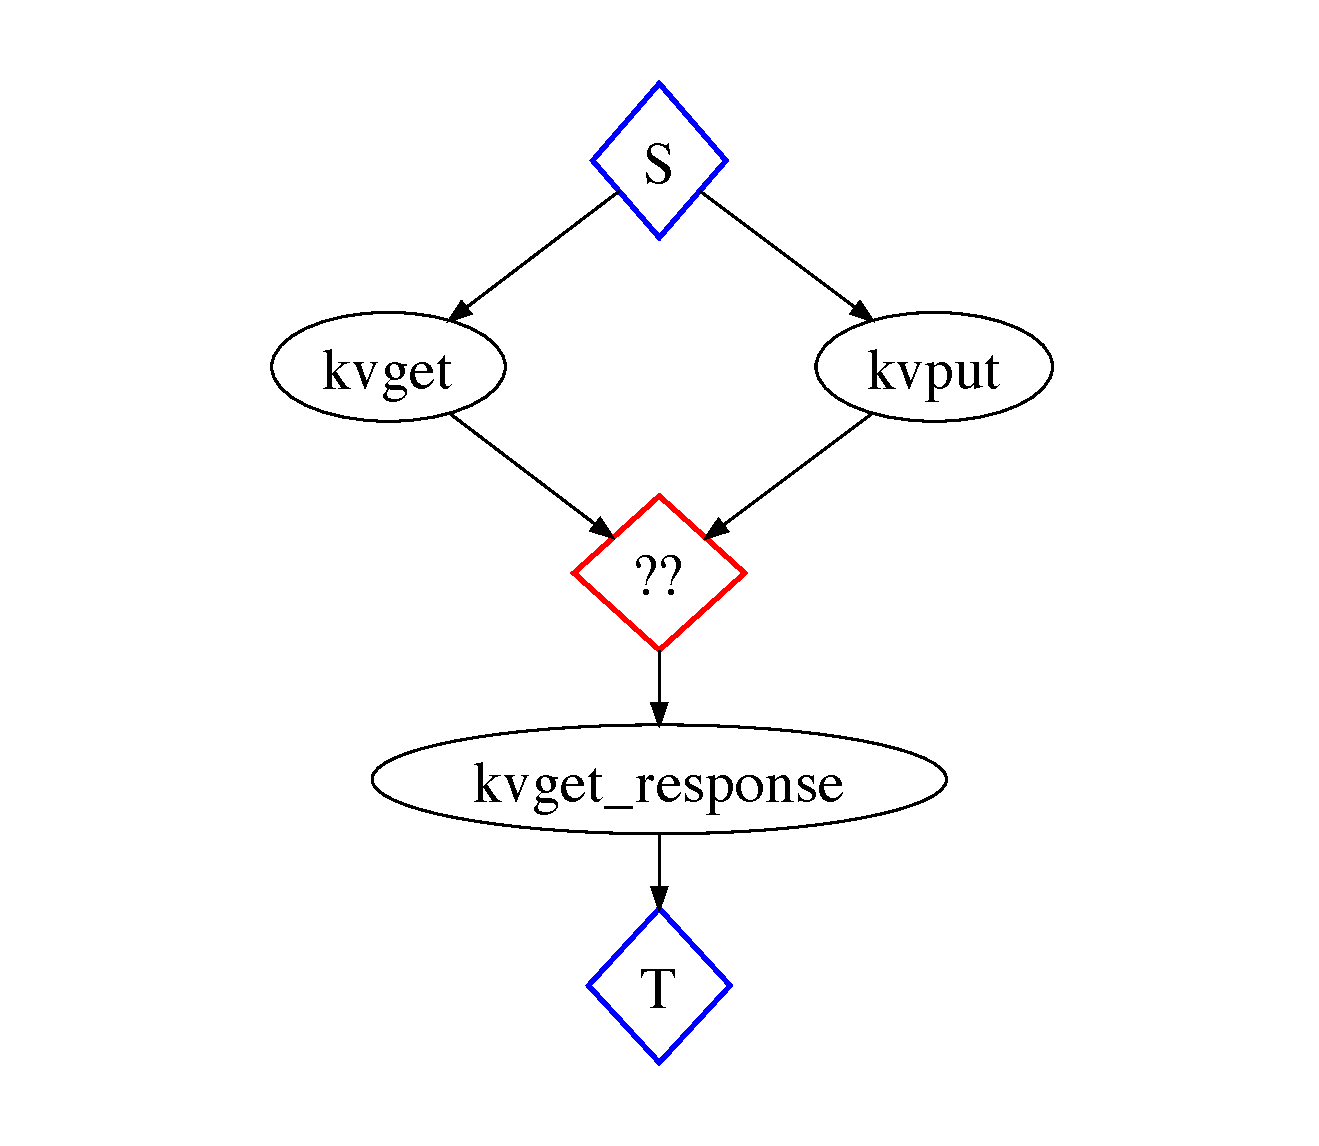
\includegraphics[width=0.4\linewidth]{fig/kvs_proto_pdg.pdf}
\vspace{-10pt}
\caption{Visualization of the abstract key-value store protocol.}
\label{fig:pdg-kvs-proto-analysis}
\vspace{-2pt}
\end{figure}

\begin{figure}[t]
\centering
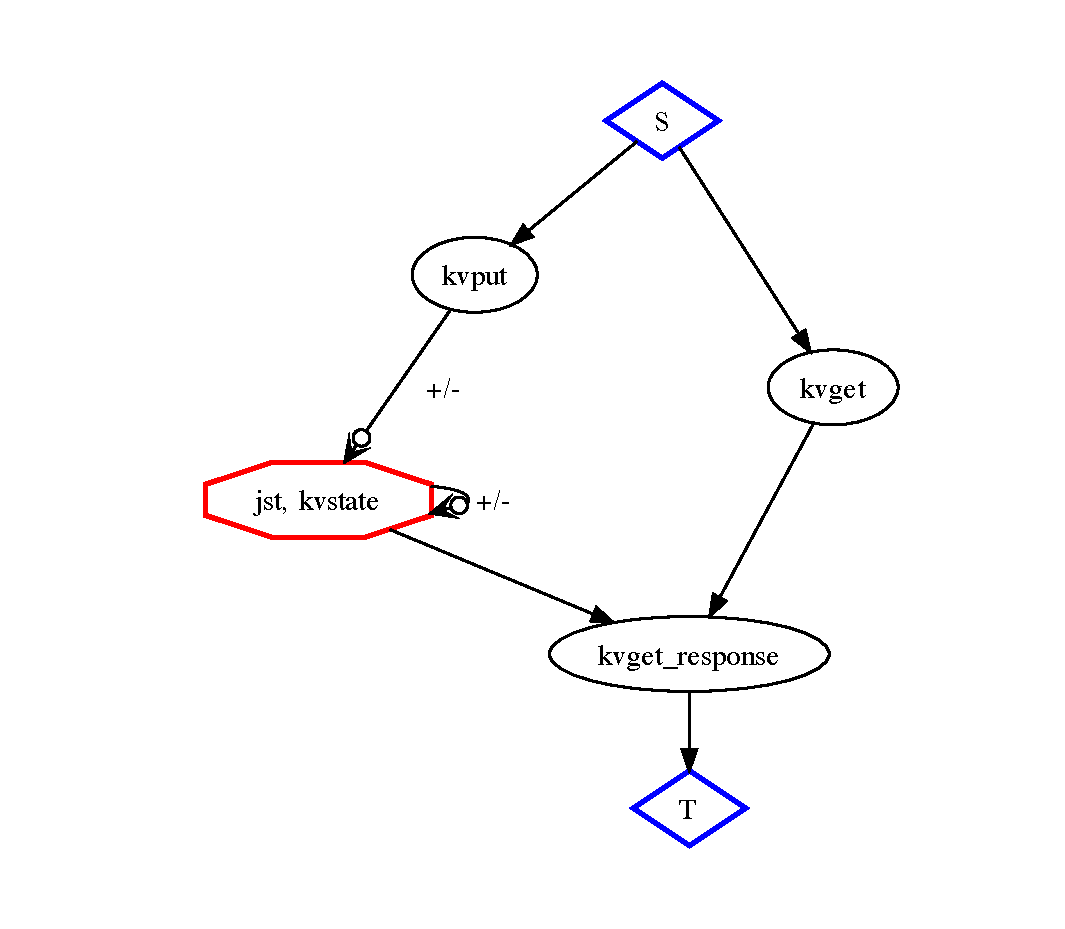
\includegraphics[width=0.5\linewidth]{fig/basickvs.pdf}
\vspace{-10pt}
\caption{Visualization of the single-site key-value store.}
\label{fig:pdg-kvs-analysis}
\vspace{-2pt}
\end{figure}
